% MNRAS manuscript, short plain-language version (v4, 2026-10-15): the v3.4 paper (MN-26-3158-P, rejected 2026-10-07) rewritten at about
% three pages plus references, every step of the algebra shown.  Build:  bash build.sh      Numbers: short_numbers.py      Figure: make_figure.py
\documentclass[fleqn,usenatbib]{mnras}
\usepackage{newtxtext,newtxmath}
\usepackage[T1]{fontenc}
\usepackage{graphicx}
\usepackage{booktabs}
\usepackage{amsmath}
\usepackage{hyperref}
\hypersetup{pdftitle={Crispy Fried Chicken Conjecture on Galaxy Dynamics}, pdfauthor={C. P. Zimmerman}}

% The corresponding author's e-mail is kept out of the public repository (see build.sh / make_upload_bundle.py of the v3 folder).
\newcommand{\authoremail}{address supplied at submission}

\title[Crispy Fried Chicken Conjecture]{Crispy Fried Chicken Conjecture on Galaxy Dynamics}

\author[C. P. Zimmerman]{Carl P. Zimmerman$^{1}$\thanks{E-mail: \authoremail}
\\
$^{1}$Briar Creek Tech, USA}

\date{Accepted XXX. Received YYY; in original form ZZZ}
\pubyear{2026}

\begin{document}
\label{firstpage}
\pagerange{\pageref{firstpage}--\pageref{lastpage}}
\maketitle

\begin{abstract}
Galaxies spin as if they feel more pull than their visible matter can supply. The extra pull appears below one special acceleration, $a_0\simeq1.2\times10^{-10}$ m s$^{-2}$. This number is close to $\tfrac12c\sqrt{G\rho_\Lambda}$, where $\rho_\Lambda$ is the density of the cosmological constant (dark energy). We call the guess $a_0=\kappa\,c\sqrt{G\rho_\Lambda}$, with $\kappa$ a pure number, the Crispy Fried Chicken conjecture, and test it with every step of the algebra shown. First, what is $\kappa$? On 175 nearby galaxies (the SPARC sample) three methods give $0.45\pm0.07$, $0.58\pm0.18$ and $0.43\pm0.08$. All agree with $1/2$, and with other simple numbers. The answer depends on how much mass each unit of starlight carries, so $1/2$ is a fitted value, not a derived one. Second, did $a_0$ change over cosmic time? If it is tied to dark energy, it did not. If it is tied to the expansion rate, it was 3.8 times larger at redshift $z=2.5$. The standard dark-matter model ($\Lambda$CDM) predicts about 1.6 times. Working out $a_0$ from one galaxy magnifies the error in its visible mass by 4 or more at the accelerations of today's distant galaxies, so they cannot decide. About eight magnified (lensed) discs at $z\simeq2.5$ would give 20:1 odds if their mass errors were independent. If the errors share a common calibration error of 0.06 dex (15 per cent), 34 are needed, and above that the sample average alone can never reach 20:1.
\end{abstract}

\begin{keywords}
gravitation -- galaxies: kinematics and dynamics -- galaxies: high-redshift -- cosmological parameters -- dark energy
\end{keywords}

\section{Introduction}
\label{sec:intro}
Stars and gas in a spinning galaxy are pulled toward its centre with acceleration $g_{\rm obs}=V^2/R$, where $V$ is their speed at distance $R$ from the centre. The visible stars and gas alone would pull less; call that smaller value $g_{\rm bar}$ (``bar'' is for baryons, meaning ordinary matter). Across thousands of measurements $g_{\rm obs}$ follows one curve of $g_{\rm bar}$ \citep{McGaugh2016,Lelli2017}. The curve has one built-in constant, an acceleration $a_0\simeq1.2\times10^{-10}$ m s$^{-2}$. Where $g_{\rm bar}\gg a_0$, $g_{\rm obs}=g_{\rm bar}$. Where $g_{\rm bar}\ll a_0$, $g_{\rm obs}\simeq\sqrt{g_{\rm bar}a_0}$. (The symbols $\gg$ and $\ll$ mean ``much larger than'' and ``much smaller than''.) \citet{Milgrom1983} proposed this as a modified law of motion (MOND) and noted that $a_0$ is about $cH_0$, where $c$ is the speed of light and $H_0$ is how fast the universe expands today. All symbols are collected in Table~\ref{tab:symbols}.

That coincidence can be read three ways. (i) $a_0$ follows the expansion rate $H(z)$, where redshift $z$ measures how far back in time we look; then $a_0$ was larger in the past. (ii) $a_0$ follows the cosmological constant, a fixed energy density of empty space (dark energy) that never changes; then $a_0$ is constant. (iii) There is no basic $a_0$. In $\Lambda$CDM, the standard cosmological model of cold dark matter plus a cosmological constant, the curve emerges from dark-matter haloes (the roughly spherical dark-matter clouds around galaxies; \citealt{Navarro2017}), whose pull also grows with redshift. Today (i) and (ii) differ by only 21 per cent, too little to measure. At $z=2.5$ they differ by a factor 3.8.

We test reading (ii). It is the \emph{Crispy Fried Chicken conjecture} (the name is the author's nickname and carries no physics), which we state in full:
\begin{enumerate}
\item[(P1)] The acceleration scale of galaxy dynamics is
\begin{equation}
a_0=\kappa\,c\sqrt{G\rho_\Lambda},
\label{eq:relation}
\end{equation}
where $G$ is Newton's constant, $\rho_\Lambda$ is the mass density of the cosmological constant, and $\kappa$ is one fixed pure number of order one.
\item[(P2)] Because $\rho_\Lambda$ never changes, $a_0$ is the same at every redshift.
\end{enumerate}
The conjecture asserts nothing about \emph{why} this holds, and it does not predict the value of $\kappa$; we fit it. It would be refuted by (R1) a measured $\kappa$ that no simple number matches, or (R2) a clear rise of $a_0$ at high redshift, $\Delta\ge+0.22$ dex with odds of 20:1 (defined in Section~\ref{sec:design}). Neither has happened: R1 is not seen (Section~\ref{sec:kappa}), and R2 cannot yet be tested (Section~\ref{sec:ztest}). It is written for a true cosmological constant. It does not differ from plain MOND with a constant $a_0$ in anything we can test today; it differs by giving the constant a source. We size differences in \emph{dex}, the power of ten: $x$ dex is a factor $10^x$, so 0.3 dex is a factor 2, 1 dex a factor 10, and 0.06 dex is 15 per cent. The paper is built as a chain. Section~\ref{sec:relation} shows by exact algebra that (P1) is the only form that units allow. Section~\ref{sec:kappa} measures $\kappa$. Section~\ref{sec:ztest} turns (P2) into a test, shows why existing galaxies cannot perform it, and says what could. Section~\ref{sec:limits} lists in a table what is and is not established. The idea is old \citep{Milgrom1999,Milgrom2020}, and \citet{Limbach2008} ran a redshift test up to $z=1.2$; we claim no priority. We do not derive $\kappa$.

\begin{table*}
\caption{Symbols. ``$\propto$'' means ``is proportional to''; ``$\simeq$'' means ``is approximately''.}
\label{tab:symbols}
\begin{tabular}{p{0.15\textwidth}p{0.33\textwidth}p{0.15\textwidth}p{0.30\textwidth}}
\toprule
symbol & meaning & symbol & meaning\\
\midrule
$g_{\rm obs}=V^2/R$ & observed pull toward the centre of a galaxy (speed $V$ at radius $R$) & $\kappa$ & the pure number in equation~(\ref{eq:relation})\\
$g_{\rm bar}$ & pull that the visible (baryonic) matter alone would give & $\Upsilon$ & mass of stars per unit of starlight, in solar units\\
$a_0$ & the special acceleration, $\simeq1.2\times10^{-10}$ m s$^{-2}$ & $\Delta(z)$ & change of $a_0$ since today, in dex (Sect.~\ref{sec:laws})\\
$y=g_{\rm bar}/a_0$ & how weak the visible pull is: $y\ll1$ is a weak pull (``deep''), $y\gg1$ a strong one & $A_{\rm obs}$, $A_{\rm bar}$ & factors that magnify errors in $g_{\rm obs}$ and in $g_{\rm bar}$ (Sect.~\ref{sec:amp})\\
$\rho_\Lambda$, $\rho_{\rm crit}$ & density of dark energy; density of a spatially flat universe & $\sigma$, $s_0$, $s_1$ & typical size (one standard deviation) of a random error\\
$H_0$, $H(z)$ & expansion rate of the universe today, and at redshift $z$ & $\delta_c$ & error shared by every galaxy's mass (dex)\\
$z$ & redshift: the larger $z$, the further back in time we look & $N$, $\ln B$ & number of galaxies; log of the odds (Sect.~\ref{sec:design})\\
\bottomrule
\end{tabular}
\end{table*}

\section{The conjecture, one step at a time}
\label{sec:relation}
\emph{Why the form is forced.} Suppose an acceleration is built from $c$, $G$ and a density $\rho$ as $a=c^{\alpha}G^{\beta}\rho^{\gamma}$. In kilograms (kg), metres (m) and seconds (s), $c$ is m s$^{-1}$, $G$ is m$^3$ kg$^{-1}$ s$^{-2}$, $\rho$ is kg m$^{-3}$ and an acceleration is m s$^{-2}$. An equation must balance in every unit, so the power of each unit must match on both sides (this is called dimensional analysis):
\begin{equation}
\begin{aligned}
\text{kg:}\quad & -\beta+\gamma=0,\\
\text{m:}\quad & \alpha+3\beta-3\gamma=1,\\
\text{s:}\quad & -\alpha-2\beta=-2 .
\end{aligned}
\label{eq:dims}
\end{equation}
The first line gives $\gamma=\beta$. Putting that into the second gives $\alpha=1$. Putting $\alpha=1$ into the third gives $\beta=1/2$. So $a=\kappa c\sqrt{G\rho}$ is the only possible form, and units cannot fix $\kappa$. Choosing $\rho=\rho_\Lambda$ is the conjecture.

\emph{The density of dark energy.} For a flat universe $H^2=8\pi G\rho/3$. Today the total density (matter plus dark energy) equals the critical density, the density of a spatially flat universe, which is what observations find. A fraction $\Omega_\Lambda$ of it is the cosmological constant:
\begin{equation}
\rho_{\rm crit}=\frac{3H_0^2}{8\pi G},\qquad \rho_\Lambda=\Omega_\Lambda\,\rho_{\rm crit}.
\label{eq:rho}
\end{equation}
Unlike matter, $\rho_\Lambda$ does not thin out as the universe expands. We use the \citet{Planck2020} values $H_0=67.4$ km s$^{-1}$ Mpc$^{-1}$ and $\Omega_\Lambda=0.685$, with 1 Mpc $=3.08568\times10^{22}$ m. Then equation~(\ref{eq:relation}) works out step by step as
\begin{equation}
\begin{aligned}
H_0&=\frac{67.4\times10^{3}}{3.08568\times10^{22}}=2.184\times10^{-18}\ {\rm s^{-1}},\\
\rho_{\rm crit}&=\frac{3H_0^2}{8\pi G}=8.533\times10^{-27}\ {\rm kg\,m^{-3}},\\
\rho_\Lambda&=0.685\,\rho_{\rm crit}=5.845\times10^{-27}\ {\rm kg\,m^{-3}},\\
\sqrt{G\rho_\Lambda}&=6.246\times10^{-19}\ {\rm s^{-1}},\\
c\sqrt{G\rho_\Lambda}&=1.872\times10^{-10}\ {\rm m\,s^{-2}} .
\end{aligned}
\end{equation}
For $\kappa=1/2$ this gives $a_0=9.36\times10^{-11}$ m s$^{-2}$. Using $\rho_{\rm crit}$ instead of $\rho_\Lambda$ makes it larger by $\Omega_\Lambda^{-1/2}=1.208$, which is $1.13\times10^{-10}$ m s$^{-2}$. Both lie inside the stated uncertainty of the usual value, $(1.20\pm0.02\pm0.24)\times10^{-10}$ m s$^{-2}$ \citep{McGaugh2016}.

\section{Measuring $\kappa$}
\label{sec:kappa}
\emph{The curve.} We use the SPARC database \citep{Lelli2016}: 175 nearby disc galaxies, each with rotation speeds measured at many radii and starlight measured at 3.6 $\mu$m. Each radius gives one point $(g_{\rm bar},g_{\rm obs})$. We keep 2803 points in 164 galaxies whose speed errors are below 10 per cent. The curve, in the form of \citet{McGaugh2016}, is an empirical formula that fits these points well; we use it only as a description,
\begin{equation}
g_{\rm obs}=\nu(y)\,g_{\rm bar},\quad \nu(y)=\frac{1}{1-e^{-\sqrt y}},\quad y\equiv\frac{g_{\rm bar}}{a_0}.
\label{eq:nu}
\end{equation}
Check the two limits. For $y\gg1$, $e^{-\sqrt y}\to0$, so $\nu\to1$ and $g_{\rm obs}=g_{\rm bar}$. For $y\ll1$, write $s=\sqrt y$ and expand $1-e^{-s}=s-s^2/2+\dots=s(1-s/2+\dots)$. (the dots are smaller terms that we drop). Then $\nu=(1/s)(1+s/2+\dots)$ and
\begin{equation}
g_{\rm obs}=\frac{g_{\rm bar}}{\sqrt y}\Big(1+\tfrac12\sqrt y\Big)=\sqrt{g_{\rm bar}a_0}\,\Big(1+\tfrac12\sqrt y\Big),
\label{eq:deep}
\end{equation}
because $g_{\rm bar}/\sqrt y=g_{\rm bar}\sqrt{a_0/g_{\rm bar}}=\sqrt{g_{\rm bar}a_0}$. The leading term says $g_{\rm obs}^2=g_{\rm bar}a_0$, that is $a_0=g_{\rm obs}^2/g_{\rm bar}$: in the weak-pull regime, $a_0$ can be read straight off the data.

\emph{Why $\kappa$ depends on the stars.} The pull $g_{\rm obs}=V^2/R$ is measured. But $g_{\rm bar}$ is computed from the light of the stars and the gas, and the stellar part is proportional to $\Upsilon$, the mass each unit of starlight carries. Nobody can measure $\Upsilon$ for a galaxy directly; it comes from models of stellar populations. Where stars dominate the visible mass, $g_{\rm bar}\propto\Upsilon$, so $a_0=g_{\rm obs}^2/g_{\rm bar}\propto1/\Upsilon$. Fitting equation~(\ref{eq:nu}) to SPARC gives $a_0=1.05$, $0.86$ and $0.71\times10^{-10}$ m s$^{-2}$, that is $\kappa=0.560$, $0.457$ and $0.381$, for $\Upsilon=0.5$, $0.6$ and $0.7$. Going from $\Upsilon=0.5$ to $0.6$ multiplies $\kappa$ by $0.457/0.560=0.82$, close to $0.5/0.6=0.83$. Stellar models give $\Upsilon=0.5$--$0.7$ \citep{Meidt2014}, and $\kappa=1/2$ needs $\Upsilon=0.555$. The scatter hardly changes (0.143--0.145 dex), so the data do not choose $\Upsilon$. One more choice matters. A galaxy's distance sets its radius $R$ and so its $g_{\rm obs}$. For 97 galaxies SPARC computes the distance from the speed at which the galaxy recedes, divided by $H_0=73$, while $\rho_\Lambda$ above uses $H_0=67.4$. We rescale those distances to 67.4 so that both sides of equation~(\ref{eq:relation}) use one $H_0$.

\emph{Three methods.} To loosen the grip of $\Upsilon$ we use three methods that depend on it differently. A: for a galaxy with weak pull, the curve implies that the speed $V_f$ in its flat outer part obeys $V_f^4\simeq GM_ba_0$, where $M_b$ is the visible mass (the baryonic Tully--Fisher relation); we measure $V_f$ and $M_b$, correct for galaxies that are not infinitely deep, and read off $a_0$, using the 24 galaxies with the weakest pull. B: only the shape of the curve. It bends where $g_{\rm bar}\sim a_0$, so the position of the bend along the $g_{\rm bar}$ axis gives $a_0$. A wrong distance scale shifts every point up or down by the same amount, so we fit with a free vertical shift and it cannot matter. C: all 3391 points, letting each galaxy choose its own $\Upsilon$. They give $\kappa=0.450\pm0.073$, $0.58\pm0.18$ and $0.43\pm0.08$ (total errors). (One $\sigma$ is one error bar; a result within about $2\sigma$ of a value is consistent with it.) Each agrees with $\kappa=1/2$ (0.7, 0.5 and $0.9\sigma$ away) and with Milgrom's $a_0=cH_\Lambda/2\pi$, which has $\kappa=0.461$ (0.1, 0.7 and $0.4\sigma$), where $H_\Lambda=H_0\sqrt{\Omega_\Lambda}$. Against this, the study of \citet{Desmond2023}, which also fits distances and inclinations, gives $\kappa=0.636\pm0.053$, $2.6\sigma$ above $1/2$. Changing the $H_0$ choice moves our three values by 0.05 to 0.10.

\emph{$\kappa$ cannot be separated from $H_0$.} Equation~(\ref{eq:rho}) gives $\sqrt{G\rho_\Lambda}=H_0\sqrt{3\Omega_\Lambda/8\pi}$, so $a_0=\kappa\,cH_0\sqrt{3\Omega_\Lambda/8\pi}$: only the product $\kappa H_0$ matters. The two current values $H_0=67.4$ and $73.04$ \citep{Riess2022} have the ratio $0.923$, and $0.4607/0.500=0.921$, so $(\kappa,H_0)=(0.500,67.4)$ and $(0.461,73.04)$ predict the same $a_0$ to $0.2$ per cent. We use $\kappa=1/2$ as a working value because it is the simplest number that fits, and for no deeper reason.

\section{Did $a_0$ change over cosmic time?}
\label{sec:ztest}
The logic of this section: the conjecture predicts no change (P2); two rivals predict a rise; so a measurement of $a_0$ at high redshift tests it. Section~\ref{sec:laws} gives the predictions, Sections~\ref{sec:amp} and 4.3 show why present data cannot make the measurement, and Section~\ref{sec:design} says what could.
\subsection{Three predictions}
\label{sec:laws}
Let $\Delta(z)\equiv\log_{10}[a_0(z)/a_0(0)]$, the change of $a_0$ since today, in dex. Here $\log_{10}x$ is the power of ten that gives $x$, so $\Delta=0.58$ means $a_0(z)=10^{0.58}a_0(0)=3.8\,a_0(0)$. \emph{(a) Tied to dark energy:} $\rho_\Lambda$ does not change, so $\Delta=0$. Plain MOND predicts the same; the dark-energy link adds a reason for it. \emph{(b) Tied to the critical density:} with $\rho_{\rm crit}(z)=3H^2(z)/8\pi G$ we get $a_0\propto H(z)$ and $\Delta=\log_{10}E(z)$, where $E(z)=H(z)/H_0=\sqrt{\Omega_m(1+z)^3+\Omega_\Lambda}$ is the standard expansion history and $\Omega_m=0.315$ is the matter share (matter was denser in the past, so $H$ was larger). At $z=2.5$,
\begin{equation}
E^2=0.315\times3.5^3+0.685=14.19,
\end{equation}
so $E=3.77$ and $\Delta=\log_{10}3.77=+0.58$. \emph{(c) Dark-matter haloes ($\Lambda$CDM):} the pull at the centre of a halo of mass $M$ and concentration $c_{200}$ (how strongly its mass is packed toward the centre) is $g_{\max}\propto(GM)^{1/3}H^{4/3}c_{200}^2/f(c_{200})$, with $f(x)=\ln(1+x)-x/(1+x)$ for the standard halo shape of \citet{NFW1997} (derivation: Appendix of \citealt{Zimmerman2026long}). At fixed $M$ the factor $H^{4/3}$ gives $\tfrac43\log_{10}E=+0.77$ at $z=2.5$, because haloes were denser; but older haloes were less concentrated, which subtracts $0.44$ \citep{DuttonMaccio2014}. The sum is $+0.33$ for $10^{12}\,{\rm M_\odot}$ and $+0.22$ for the lighter haloes of the discs of Section~\ref{sec:design}; across halo mass and model \citep{Duffy2008}, $+0.17$ to $+0.56$.

\begin{figure*}
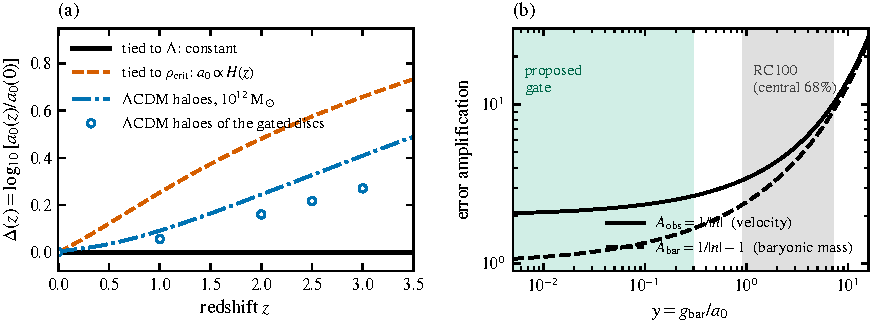
\includegraphics[width=\textwidth]{fig1_laws_amplification.pdf}
\caption{(a) The three predictions of Section~\ref{sec:laws}. The circles are the $\Lambda$CDM rise for the haloes of the discs selected by the gate of Section~\ref{sec:design}. (b) How many times an error in the observed pull ($A_{\rm obs}$) and in the visible mass ($A_{\rm bar}$) is magnified when $a_0$ is worked out from one galaxy (equation~\ref{eq:amp}). Green: the proposed gate, $y<0.3$. Grey: the central 68 per cent of the RC100 sample.}
\label{fig:laws}
\end{figure*}

\subsection{Why one galaxy tells you so little}
\label{sec:amp}
Take one galaxy at one radius, with measured $g_{\rm obs}$ and $g_{\rm bar}$. Solve $\nu(y)=g_{\rm obs}/g_{\rm bar}$ for $y$, and set $\hat a_0=g_{\rm bar}/y$ (the hat means ``estimated''). If $g_{\rm obs}$ and $g_{\rm bar}$ carry errors, how large is the error in $\hat a_0$? Below, $\ln$ is the natural logarithm and ${\rm d}\ln x$ means a tiny fractional change of $x$ (${\rm d}\ln x=0.01$ is a 1 per cent change).
\begin{enumerate}
\item Take the logarithm of $g_{\rm obs}=\nu(y)g_{\rm bar}$: $\ln\nu(y)=\ln g_{\rm obs}-\ln g_{\rm bar}$.
\item Make small changes. With $n\equiv{\rm d}\ln\nu/{\rm d}\ln y$: $n\,{\rm d}\ln y={\rm d}\ln g_{\rm obs}-{\rm d}\ln g_{\rm bar}$.
\item From $\hat a_0=g_{\rm bar}/y$: ${\rm d}\ln\hat a_0={\rm d}\ln g_{\rm bar}-{\rm d}\ln y$.
\item Put ${\rm d}\ln y$ from step 2 into step 3:
\begin{equation}
{\rm d}\ln\hat a_0=-\frac1n\,{\rm d}\ln g_{\rm obs}+\Big(1+\frac1n\Big){\rm d}\ln g_{\rm bar}.
\label{eq:amp}
\end{equation}
\item For equation~(\ref{eq:nu}), $\ln\nu=-\ln(1-e^{-s})$ with $s=\sqrt y$, so ${\rm d}\ln\nu/{\rm d}s=-1/(e^{s}-1)$. With ${\rm d}\ln y=2\,{\rm d}s/s$,
\begin{equation}
n=-\frac{\sqrt y/2}{e^{\sqrt y}-1}.
\end{equation}
\end{enumerate}
Here $n<0$, so define $A_{\rm obs}=1/|n|$ and $A_{\rm bar}=A_{\rm obs}-1$. A fractional error $\epsilon$ in $g_{\rm obs}$ becomes $A_{\rm obs}\epsilon$ in $\hat a_0$, and one in $g_{\rm bar}$ becomes $A_{\rm bar}\epsilon$. For small $y$, $n\to-1/2$, so $A_{\rm obs}=2$ and $A_{\rm bar}=1$. Both grow with $y$ (Fig.~\ref{fig:laws}b): $A_{\rm bar}=1.1$ at $y=0.01$, $1.7$ at $y=0.3$, $3.8$ at $y=2.4$ and $8.1$ at $y=6.4$. The reason: where the pull is strong, $g_{\rm obs}\simeq g_{\rm bar}$ whatever $a_0$ is, so a small error in the data moves the inferred $a_0$ a lot. Errors are least harmful where the pull is weak.

\subsection{What existing data say}
The largest uniform sample of distant galaxies, RC100 \citep[100 rotation curves of star-forming discs, $0.6<z<2.5$]{NestorShachar2023}, takes visible masses from starlight plus gas masses estimated from scaling relations, that is, average gas-to-star ratios measured in other galaxies \citep{Tacconi2018}. Its median (middle value) is $y=2.4$ and its central 68 per cent (the middle two thirds of the galaxies) lies in $0.9<y<7.2$. At the median $A_{\rm bar}=3.8$, so a typical $0.2$ dex error in visible mass becomes $0.76$ dex in $a_0$, larger than any gap in Fig.~\ref{fig:laws}a. For 41 of the 100 discs the estimated visible pull already equals or exceeds the observed pull ($g_{\rm bar}\ge g_{\rm obs}$), which the curve cannot produce, so no $a_0$ can be worked out (27 per cent of discs at $z<1$, 51 per cent at $z>2$). RC100 therefore measures how well visible masses are known, not $a_0$. The rise at $z\simeq1$ reported by \citet{Ciocan2026} appears when disc masses are fitted together with a dark halo and not when they come from starlight (\citealt{Zimmerman2026long}, Sect.~4.3), so we count it neither way. No existing sample decides.

\subsection{What would decide}
\label{sec:design}
\emph{The gate.} The gate is a rule for which galaxies to include: only discs whose visible pull at their outermost radius is $g_{\rm bar}<0.3a_0$, where $A_{\rm obs}\le2.7$ and $A_{\rm bar}\le1.7$. A point mass $M_b$ would pull with $GM_b/R^2$; a disc pulls somewhat more, by a shape factor $\Gamma\simeq1.2$. So $g_{\rm bar}=\Gamma GM_b/R^2$ and the limit on the visible mass $M_b$ is
\begin{equation}
\begin{aligned}
M_b&<\frac{0.3\,a_0R^2}{\Gamma G}=\frac{0.3\,(9.36\times10^{-11})(3.086\times10^{19})^2}{1.2\,(6.674\times10^{-11})}\ {\rm kg}\\
&=1.7\times10^{8}\,{\rm M_\odot}\,(R/{\rm kpc})^2,
\end{aligned}
\end{equation}
using 1 kpc (kiloparsec) $=3.086\times10^{19}$ m and one solar mass ${\rm M_\odot}=1.989\times10^{30}$ kg. At $z\simeq2.5$ such small discs can be resolved only when a foreground galaxy magnifies them (gravitational lensing), and their gas mass must be measured, not guessed.

\emph{How many galaxies?} Each galaxy gives one measured value $x=\Delta_i$ of the change of $a_0$. We compare two predictions for it, $0$ (constant $a_0$) and $\Delta$ (a rise). Odds of 20:1 mean that the data are 20 times more likely under one prediction than under the other, which is conventionally called strong evidence \citep{KassRaftery1995}. Suppose the measurement error is Gaussian (a bell-curve scatter) of size $\sigma$. The log of the likelihood ratio, that is of the odds $B$ for prediction $\Delta$ against $0$, is $[x^2-(x-\Delta)^2]/2\sigma^2=(2x\Delta-\Delta^2)/2\sigma^2$. If $\Delta$ is true, the average of $x$ over many repeats is $\Delta$, so the expected value (written $\langle\cdot\rangle$) is $\langle\ln B\rangle=\Delta^2/2\sigma^2$. Independent galaxies add their logs, so $N$ galaxies give $N\Delta^2/2\sigma^2$. Odds of 20:1 need $N\Delta^2/2\sigma^2=\ln20$, that is
\begin{equation}
\frac{\sigma}{\sqrt N}\le\frac{\Delta}{\sqrt{2\ln20}}=\frac{\Delta}{2.45}.
\end{equation}
So the sample mean must be known to $0.216/2.45=0.088$ dex to test against the $\Lambda$CDM rise of the gated discs, and to $0.576/2.45=0.24$ dex against $H(z)$. A fuller count notes that the two predictions also differ in spread: $s_0^2=\sigma_{\rm m}^2+\sigma_{\rm int}^2$ if $a_0$ is constant, and $s_1^2=s_0^2+\sigma_{\rm h}^2$ for haloes. Here $\sigma_{\rm m}$ is the measurement error, $\sigma_{\rm int}=0.034A_{\rm obs}(0.3)=0.09$ dex is the natural scatter of the curve, and $\sigma_{\rm h}=0.135$ dex is the scatter between haloes. If $a_0$ is constant, each galaxy then adds
\begin{equation}
\ln\frac{s_1}{s_0}-\frac12+\frac{s_0^2+\Delta^2}{2s_1^2}
\end{equation}
to $\langle\ln B\rangle$ (the less favourable case; if the haloes are right it is larger, 0.513 below). For $\sigma_{\rm m}=0.20$ dex, $s_0=0.2195$ and $s_1=0.2575$, so each galaxy adds $0.375$: eight galaxies give $e^{8\times0.375}=20:1$ and seven give $14:1$. Expected odds are not the chance of reaching them. By Monte Carlo (repeating the experiment many times on a computer with random errors), that chance is 0.53 for eight galaxies, and 20 are needed for 0.9.

\emph{A shared calibration error does not average down.} Part of the mass error is the same for every galaxy (for example the conversion from carbon-monoxide (CO) light to gas mass, or the stellar-mass zero point). A shared error $\delta_c$ (in dex) adds the same $\sigma_C=A_{\rm bar}\delta_c$ to every $\Delta_i$, so the variance of the sample mean is $s^2/N+\sigma_C^2$, which stops falling at $\sigma_C^2$. Using $\sigma_C$ in place of $\sigma/\sqrt N$ above, odds of 20:1 from the means need $\delta_c\le\Delta/(2.45\,A_{\rm bar})$. At $y=0.2$, $A_{\rm bar}=1.52$, so
\begin{equation}
\begin{aligned}
\delta_c&\le\frac{0.216}{2.45\times1.52}=0.058\ \text{dex (haloes)},\\
\delta_c&\le\frac{0.576}{2.45\times1.52}=0.155\ \text{dex ($H(z)$)}.
\end{aligned}
\end{equation}
Beyond these limits the sample average alone can never reach 20:1, however many galaxies are used. (The spread of the sample also differs between the two predictions and adds some information: at $\delta_c=0.07$ dex, 52 galaxies would give 20:1.) Below the limits the number needed rises, from eight at $\delta_c=0$ to 14, 20 and 34 at $\delta_c=0.04$, $0.05$ and $0.06$ dex. Deep galaxies cannot fit this calibration themselves: if every mass is multiplied by $f$, then $g_{\rm bar}\to fg_{\rm bar}$ and $g_{\rm obs}^2=g_{\rm bar}a_0$ becomes $g_{\rm obs}^2=g_{\rm bar}(fa_0)$, so they measure only the product $fa_0$. The calibration must come from outside the rotation curves, in practice from gas masses measured galaxy by galaxy. The test is the mean of the $\Delta_i$ over the gated galaxies. Near 0 it supports a constant $a_0$; near $+0.22$ or above, an emergent or $H(z)$-tied scale; and if it fits none of them, it counts against all.

\section{What is and is not established}
\label{sec:limits}
Table~\ref{tab:ledger} separates exact algebra, fits, predictions and open questions.

\begin{table*}
\caption{What this paper establishes, claim by claim.}
\label{tab:ledger}
\begin{tabular}{p{0.46\textwidth}p{0.4\textwidth}l}
\toprule
claim & status & where\\
\midrule
For any density, units allow only $a=\kappa c\sqrt{G\rho}$ & exact algebra & Sect.~\ref{sec:relation}\\
For $\kappa=1/2$ and $\rho_\Lambda$, $a_0=9.36\times10^{-11}$ m s$^{-2}$, inside the measured range & arithmetic, recomputed by script & Sect.~\ref{sec:relation}\\
$\kappa\simeq1/2$ fits nearby galaxies & fits; but $\kappa$ is fitted, depends on $\Upsilon$ and $H_0$, and one study is $2.6\sigma$ away & Sect.~\ref{sec:kappa}\\
$\kappa=1/2$ follows from a deeper principle & not shown; nothing here derives it & ---\\
$a_0$ is constant in time (P2) & a prediction; untested & Sect.~\ref{sec:laws}\\
Existing distant galaxies can test (P2) & no: their errors are magnified 4 to 8 times & Sects.~\ref{sec:amp}--4.3\\
A specified measurement can test (P2) & yes: about 8 to 34 lensed discs with measured gas masses & Sect.~\ref{sec:design}\\
Galaxies need modified gravity rather than dark matter & not addressed & ---\\
\bottomrule
\end{tabular}
\end{table*}

\emph{$\kappa$ is not derived:} it is fitted, and $0.461$ fits as well. \emph{A number is not a mechanism:} equation~(\ref{eq:relation}) fixes a value, not whether galaxies need modified gravity, modified inertia or dark matter, and it does not remove the need for the cold matter measured by the microwave background. If dark energy evolves \citep{DESI2025}, $a_0\propto\sqrt{\rho_{\rm DE}}$ would change by only about $-0.1$ dex at $z=2.5$. In plain words: the number $1/2$ fits nearby galaxies but nothing derives it; today's distant galaxies are too imprecise to say whether $a_0$ has changed; and what is missing for a decision is gas mass measured galaxy by galaxy at $z\simeq2.5$, in about eight to thirty-four carefully chosen lensed discs.

\section*{Acknowledgements}
Generative AI tools were used. Large language models assisted with code, literature checks, transcribing published data and drafting the text: Anthropic's Claude (mainly via Claude Code, which also rewrote this short version), and models from OpenAI, DeepSeek, Zhipu AI (GLM), Alibaba (Qwen), Google (Gemini, Gemma), Tencent (Hunyuan), Moonshot AI (Kimi) and xAI (Grok). The author checked every result, has reviewed the full content and takes sole responsibility for it. We used the SPARC database \citep{Lelli2016} and the table of \citet{NestorShachar2023}. No funding; no conflict of interest.

\section*{Data Availability}
Every number is produced by \texttt{short\_numbers.py} (figure: \texttt{make\_figure.py}) in \url{https://github.com/carlzimmerman/zimmerman-formula}, directory \nolinkurl{qwen_claude_field_theory/papers_2026/mnras_submission_2026_v4_short}. Measured quantities are read from the committed outputs of the longer analysis (\nolinkurl{mnras_submission_2026_v3}, tag \texttt{mnras-v3.4}; \citealt{Zimmerman2026long}). SPARC: \url{http://astroweb.cwru.edu/SPARC/}.

\bibliographystyle{mnras}
\bibliography{references}

\bsp
\label{lastpage}
\end{document}
